
\documentclass[a4paper,11pt]{article}

\usepackage[T1]{fontenc}
\usepackage[utf8]{inputenc}
\usepackage{graphicx}
\usepackage{xcolor}

\renewcommand\familydefault{\sfdefault}
\usepackage{tgheros}
\usepackage[defaultmono]{droidmono}

\usepackage{amsmath,amssymb,amsthm,textcomp}
\usepackage{enumerate}
\usepackage{multicol}
\usepackage{tikz}

\usepackage{geometry}
\geometry{total={210mm,297mm},
left=25mm,right=25mm,%
bindingoffset=0mm, top=20mm,bottom=20mm}


\linespread{1.3}

\newcommand{\linia}{\rule{\linewidth}{0.5pt}}

% custom theorems if needed
\newtheoremstyle{mytheor}
    {1ex}{1ex}{\normalfont}{0pt}{\scshape}{.}{1ex}
    {{\thmname{#1 }}{\thmnumber{#2}}{\thmnote{ (#3)}}}

\theoremstyle{mytheor}
\newtheorem{defi}{Definition}

% my own titles
\makeatletter
\renewcommand{\maketitle}{
\begin{center}
\vspace{2ex}
{\huge \textsc{\@title}}
\vspace{1ex}
\\
\linia\\
\@author \hfill \@date
\vspace{4ex}
\end{center}
}
\makeatother
%%%

% custom footers and headers
\usepackage{fancyhdr}
\pagestyle{fancy}
\lhead{}
\chead{}
\rhead{}
\lfoot{SimTools Project 1}
\cfoot{}
\rfoot{Page \thepage}
\renewcommand{\headrulewidth}{0pt}
\renewcommand{\footrulewidth}{0pt}
%

% code listing settings
\usepackage{listings}
\lstset{
    language=Python,
    basicstyle=\ttfamily\small,
    aboveskip={1.0\baselineskip},
    belowskip={1.0\baselineskip},
    columns=fixed,
    extendedchars=true,
    breaklines=true,
    tabsize=4,
    prebreak=\raisebox{0ex}[0ex][0ex]{\ensuremath{\hookleftarrow}},
    frame=lines,
    showtabs=false,
    showspaces=false,
    showstringspaces=false,
    keywordstyle=\color[rgb]{0.627,0.126,0.941},
    commentstyle=\color[rgb]{0.133,0.545,0.133},
    stringstyle=\color[rgb]{01,0,0},
    numbers=left,
    numberstyle=\small,
    stepnumber=1,
    numbersep=10pt,
    captionpos=t,
    escapeinside={\%*}{*)}
}

%%%----------%%%----------%%%----------%%%----------%%%

\begin{document}

\title{Simulation Tools FMNN05 \\Project 1}

\author{Nils Fagerberg, Daniel Odenbrand, Felicia Seemann and Linus Jangland}

\date{\today}

\maketitle

\section*{Background}
As a part of the course Simulation Tools, FMNN05, at LTH there are three projects related to simulating solutions of differential equations using the tools Assimulo/Sundials, Dymola/Modelica and the programming language Python. 

Every project is divided into smaller tasks. We will present each task followed by its results one by one. This is the report for project 1.

\section*{Task 1}
Task 1 consisted of a model for an elastic pendulum given by the following ODE
\begin{align}
& \dot{y_1} = y_3 \\
& \dot{y_2} = y_4 \\
& \dot{y_3} = -y_1 \cdot \lambda (y_1, y_2) \\
& \dot{y_4} = -y_1 \cdot \lambda (y_1, y_2)  - 1
\end{align}

where $\lambda (y_1, y_2) = k \frac{\sqrt{y_1^2 + y_2^2} - 1}{\sqrt{y_1^2 + y_2^2}}$. This corresponds to a mathematical pendulum where the bar is replaced by a linear spring with spring constant $k$. The mass-, nominal pendulum length and gravitational constant are taken to be one.

The task is to set up this problem in Python and solve it using Assimulo.

\subsection*{Solution}
The code for task 1 can be viewed below:

\begin{lstlisting}[caption=Script for solving Task 1]
#lambda(y1, y2, k)
def lambda_func(y1, y2, k = 1):
    return k*(np.sqrt(y1**2 + y2**2) - 1)/np.sqrt(y1**2 + y2**2)

#the right hand side of our problem
def rhs(t, y):
    return np.array([y[2], y[3], -y[0]*lambda_func(y[0], y[1]), -y[1]*lambda_func(y[0], y[1]) - 1])

#initial values. y[0] = x-position, y[1] = y-position, y[2] = x-velocity, y[3] = y-velocity
y0 = np.array([1.0, 0.0, 0.0, -1.0])
t0 = 0.0

#Assimulo stuff
model = Explicit_Problem(rhs, y0, t0)
model.name = 'Task 1'
sim = CVode(model)
sim.maxord = 7
tfinal = 100.0
#simulation. Store result in t and y
t, y = sim.simulate(tfinal)

#Create plots. Three figures are created: one containing positional values as a function of time, one with velocities as a function of time and the last traces the pendulum's movement (x and y coordinates in cartesian coordinate)
fig, ax = plt.subplots()
ax.plot(t, y[:, 0], label='x-pos')
ax.plot(t, y[:, 1], label='y-pos')
legend = ax.legend(loc='upper center', shadow=True)

plt.figure(1)
fig2, ax2 = plt.subplots()
ax2.plot(t, y[:, 2], label='x-vel')
ax2.plot(t, y[:, 3], label='y-vel')
legend = ax2.legend(loc='upper center', shadow=True)

plt.figure(1)
fig3, ax3 = plt.subplots()
ax3.plot(y[:, 0], y[:, 1], label='displacement')
legend = ax3.legend(loc='upper center', shadow=True)

# Now add the legend with some customizations.
plt.show()
\end{lstlisting}

We use the solver CVode.

%\newpage
\subsection*{Results}
Below some resulting plots of our implementation can be seen. All plots are in the time-interval 0 to 20 and the initial values are all zeros except for the $x$ which is set to 1 without elongations since the pendulum length is 1.

\begin{figure}[!h]
\centering
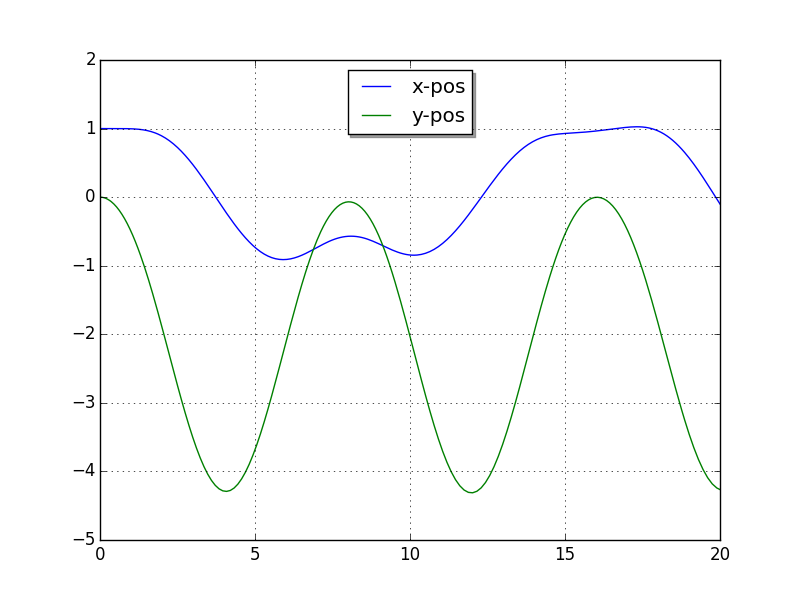
\includegraphics[scale=0.5]{task1_k075_1.png}
\caption{x and y positions as functions of time, with $k = 0.75$}
\label{1k075}
\end{figure}

\begin{figure}[!h]
\centering
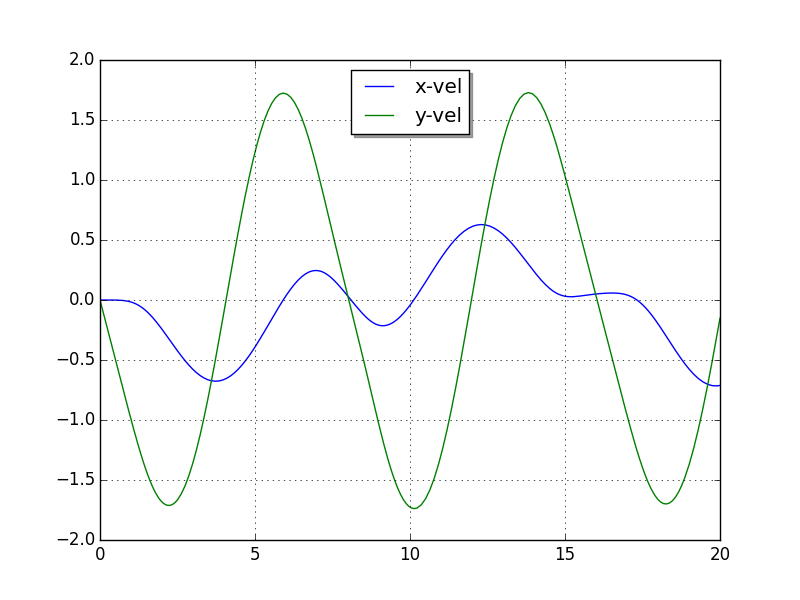
\includegraphics[scale=0.5]{task1_k075_2.png}
\caption{velocities in x- and y-directions as functions of time, with $k = 0.75$}
\label{2k075}
\end{figure}

\begin{figure}[!h]
\centering
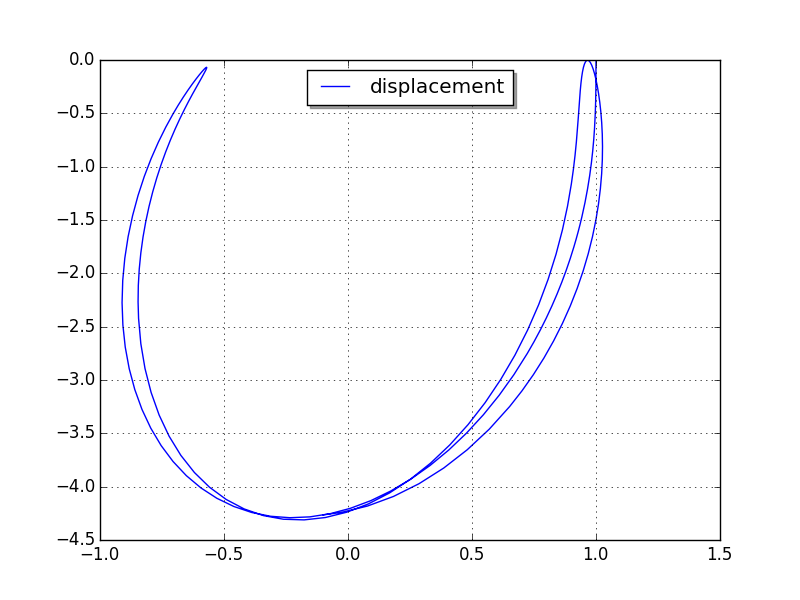
\includegraphics[scale=0.5]{task1_k075_3.png}
\caption{tracings of the pendulum trajectory for $k = 0.75$}
\label{3k075}
\end{figure}

In figures \ref{1k075}, \ref{2k075} and \ref{3k075} we have used the spring constant $k = 0.75$ which is very elastic as seen specifically in figure \ref{3k075} where the pendulum does an irregular motion. The y-position varies between 0 and about -4 and the x-position varies between 1 and -1 according to figure \ref{1k075}. Also the y-velocity is more regular than the x-velocity, as seen in figure \ref{2k075}.

\begin{figure}[!h]
\centering
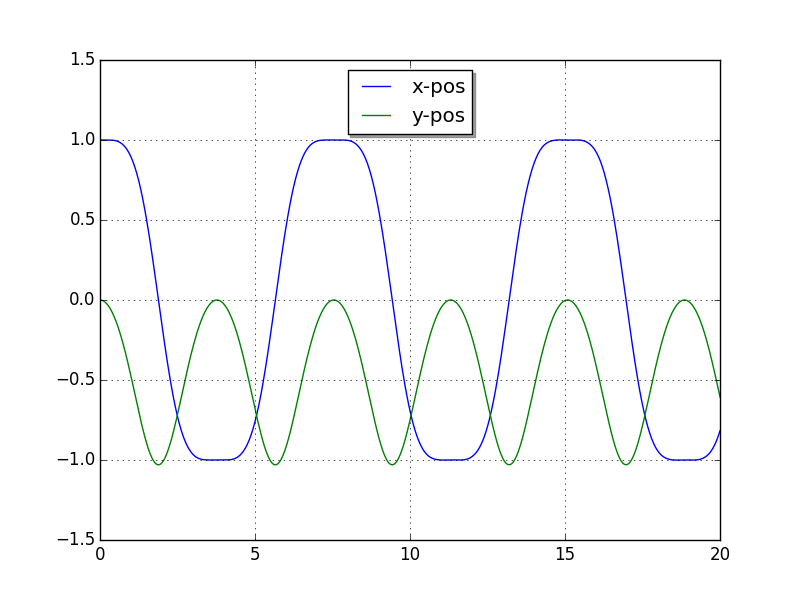
\includegraphics[scale=0.5]{task1_k100_1.png}
\caption{x and y positions as functions of time, with $k = 100$}
\label{1k100}
\end{figure}

\begin{figure}[!h]
\centering
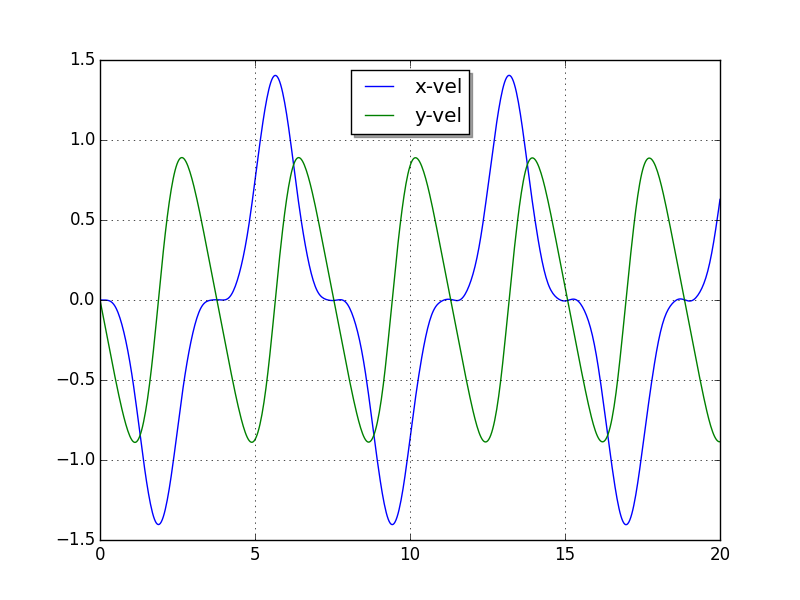
\includegraphics[scale=0.5]{task1_k100_2.png}
\caption{velocities in x- and y-directions as functions of time, with $k = 100$}
\label{2k100}
\end{figure}

\begin{figure}[!h]
\centering
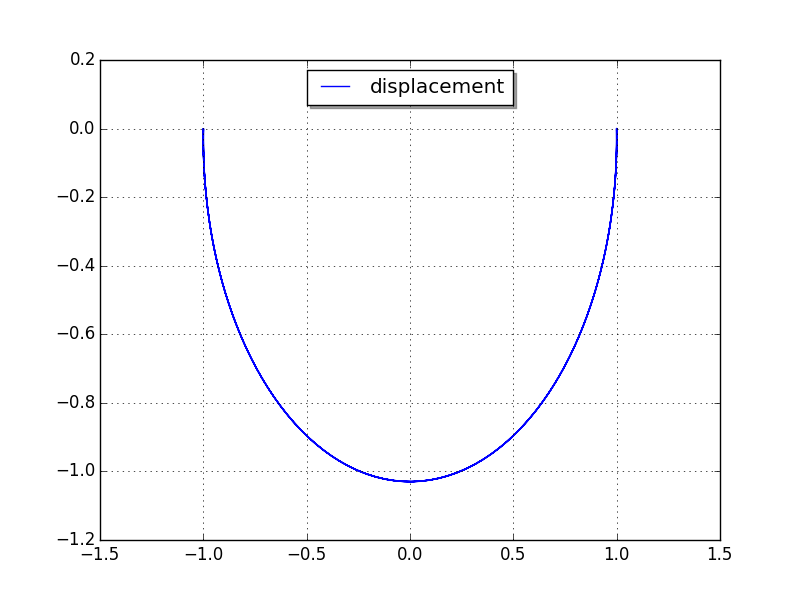
\includegraphics[scale=0.5]{task1_k100_3.png}
\caption{tracings of the pendulum trajectory for $k = 100$}
\label{3k100}
\end{figure}

In contrast, figures \ref{1k100}, \ref{2k100} and \ref{3k100} display results of a more stiff pendulum ($k = 100$). As is visible in figure \ref{3k100}, the pendulum trajectory is uniform and rather unexciting. The positional values and velocities are very periodic as you would expect from e.g. a grandfather clock.

\begin{figure}[!h]
\centering
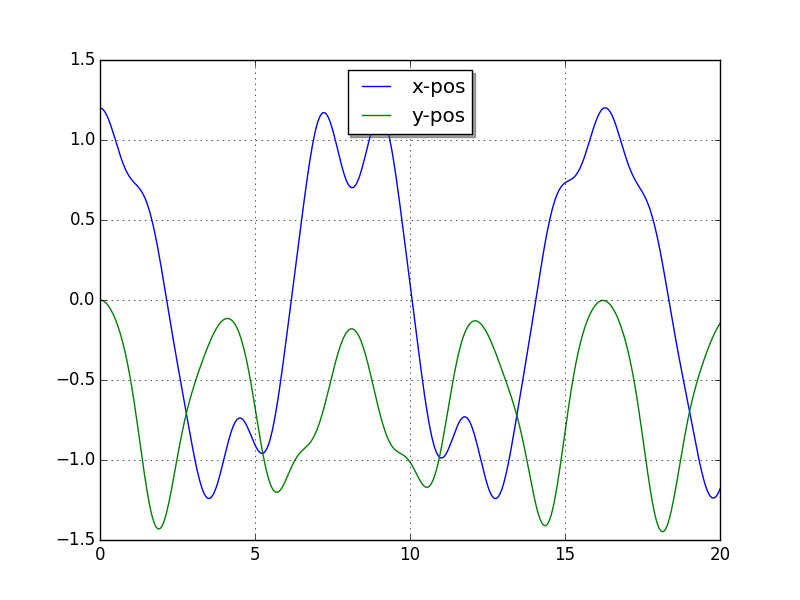
\includegraphics[scale=0.5]{task1_k10_utdrag12_1.png}
\caption{x and y positions as functions of time, with $k = 10$}
\label{1k10}
\end{figure}

\begin{figure}[!h]
\centering
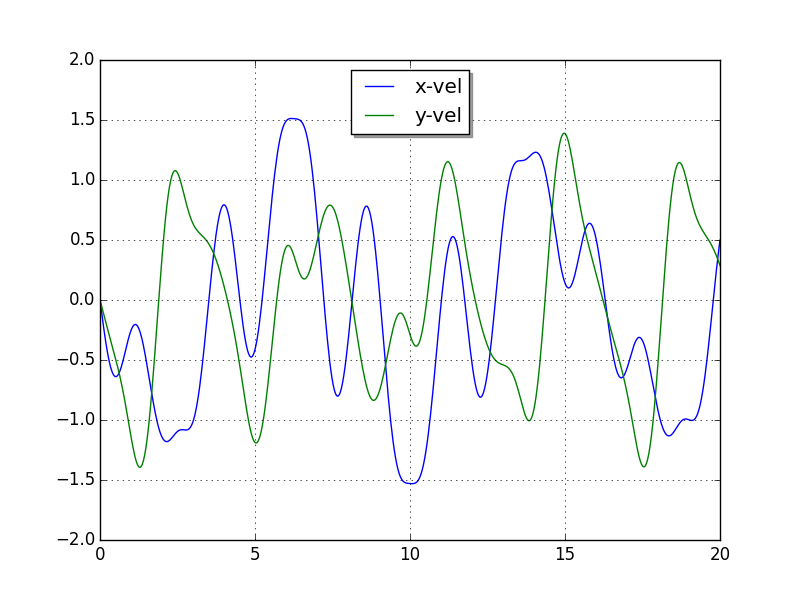
\includegraphics[scale=0.5]{task1_k10_utdrag12_2.png}
\caption{velocities in x- and y-directions as functions of time, with $k = 10$}
\label{2k10}
\end{figure}

\begin{figure}[!h]
\centering
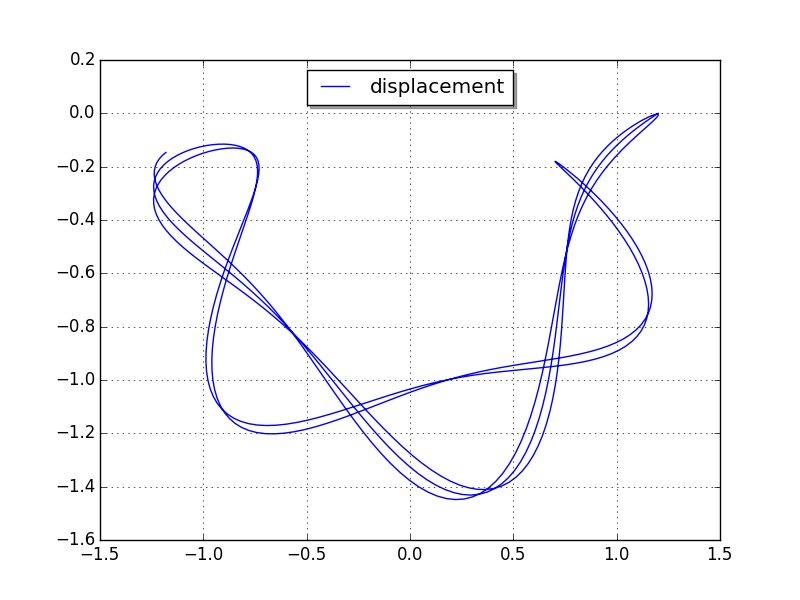
\includegraphics[scale=0.5]{task1_k10_utdrag12_3.png}
\caption{tracings of the pendulum trajectory for $k = 10$}
\label{3k10}
\end{figure}

To obtain an oscillation around the trajectory of a stiff pendulum we can start with an elongation of the spring (we used $x = 1.2$ as initial value) which would result in the pendulum contracting. Some plots of this are visible in figures \ref{1k10}, \ref{2k10} and \ref{3k10}. We can also see that the y-position and y-velocity values are a bit more irregular.

\subsection*{Discussion}
We can see that the spring is very elastic in figure \ref{3k075} since the pendulum is stretched out about 4 times its original size. Despite this, we observe a very low disturbance in the y-position and y-velocity's periodicities. This is due to the force from the spring being much lower than the gravitational force acting on the pendulum. The x-values, however are unaffected by gravity, resulting in a visible effect. This hypothesis is reinforced by the figures from the stiff pendulum, where $k = 100$, in which the x-values also become very periodic.

With a initial elongation of the spring we would expect the y-values to become more irregular since the spring is oscillating around its equilibrium.

\section*{Task 2}
Our implementations of BDF-4 and BDF-3 can be seen below:


\section*{Task 3}
%insert experiments with different methods

\section*{Task 4}
Now we repeat the experiments from task 3 using the solver CVode again. We also test the influence of ATOL, RTOL, MAXORD and the choice of discretization on the performance for the low and highly oscillating case.

\subsection*{Low oscillation}
Here we will test different parameters using $k = 10$ and the initial elongation $x = 1.2$, for a low oscillation.

\subsubsection*{ATOL and RTOL}
%SKRIV NÅT VETTIGT om atol vs rtol 


Both of these options concern error tolerances and are therefore discussed together. Having a higher tolerance will allow the solver to take larger steps, thus making the solution look choppy, as seen in figure \ref{3k10at01}.

\begin{figure}[!h]
\centering
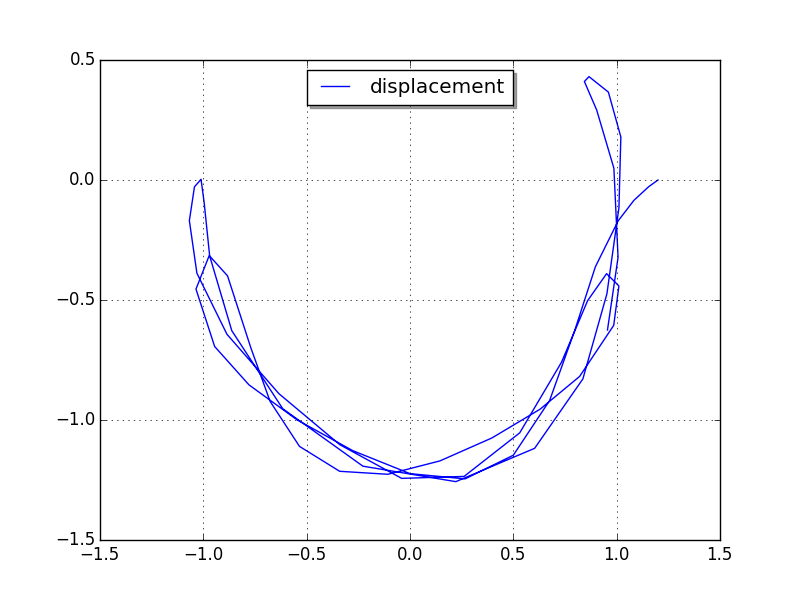
\includegraphics[scale=0.5]{task1_k10_utdrag12_atol01.png}
\caption{tracings of the pendulum trajectory for $k = 10$ with $atol = 1$}
\label{3k10at01}
\end{figure}

\begin{figure}[!h]
\centering
\includegraphics[scale=0.5]{task1_k10_utdrag12_rtol01.png}
\caption{tracings of the pendulum trajectory for $k = 10$ with $rtol = 1$}
\label{3k10rt01}
\end{figure}

\subsubsection*{MAXORD}
The maximum order of a method determines the number of past points that are used as reference for approximating the next value. A high order method will have the potential for taking larger steps at the cost of more computations per step. To ensure the same accuracy with a lower order method we must take smaller steps. For example running our code from task 1 using the order 1 takes 38501 steps, compared to the 536 steps taken using the default order (12).

\subsubsection*{Choice of discretization}
We compared both discretization using Adams method and the BDF method. Both methods generated a displacement-graph which were very much simular to each other. There are some differences in the number of steps and evaluation that both methods use, but the run-times are practically the same (Adams is slightly faster).

\subsection*{High oscillation}
Now  we test the different parameters' influence in the highly oscillating case, using $k = 50$ and initial elongation $x = 1.2$.

\subsubsection*{ATOL and RTOL}

%SKRIV NÅ VETTIGT

\begin{figure}[!h]
\centering
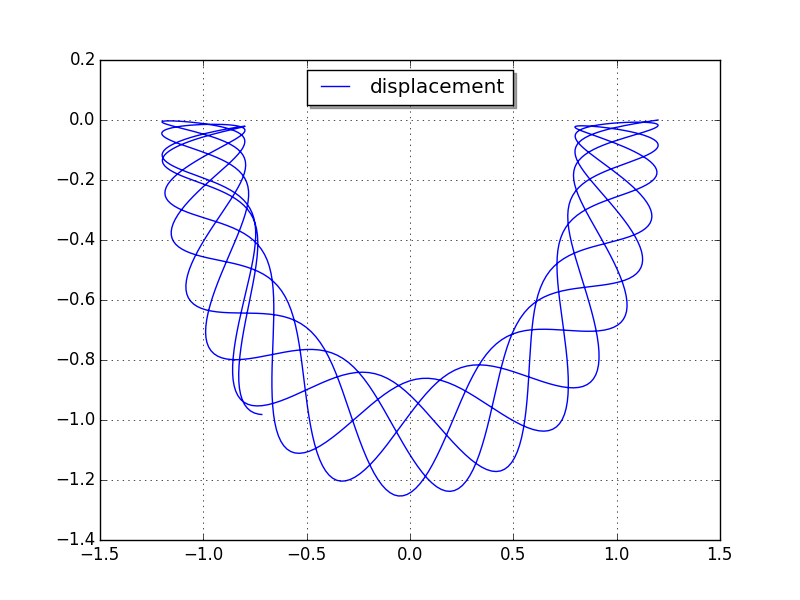
\includegraphics[scale=0.5]{task1_k50_utdrag12_default.png}
\caption{tracings of the pendulum trajectory for $k = 50$ with default a- and rtol}
\label{3k10at01}
\end{figure}

\begin{figure}[!h]
\centering
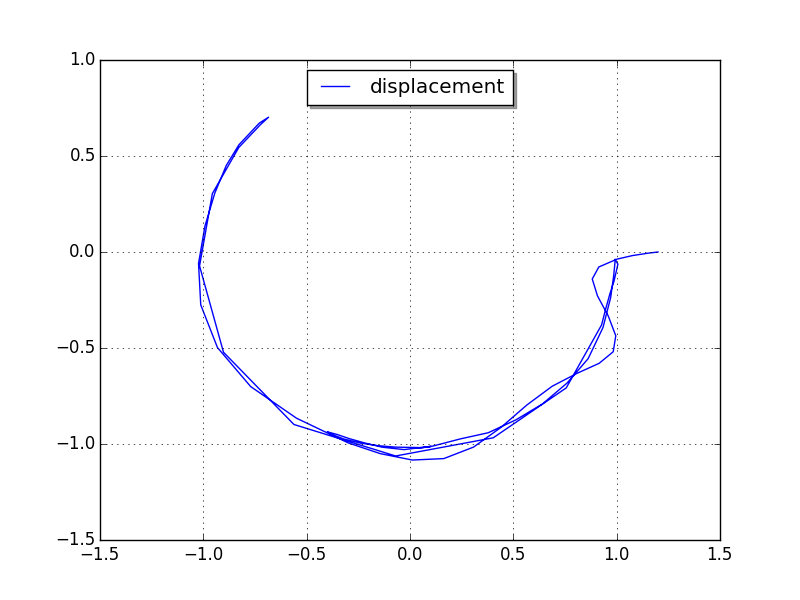
\includegraphics[scale=0.5]{task1_k50_utdrag12_atol01.png}
\caption{tracings of the pendulum trajectory for $k = 50$ with $rtol = 1$}
\label{3k10rt01}
\end{figure}

\begin{figure}[!h]
\centering
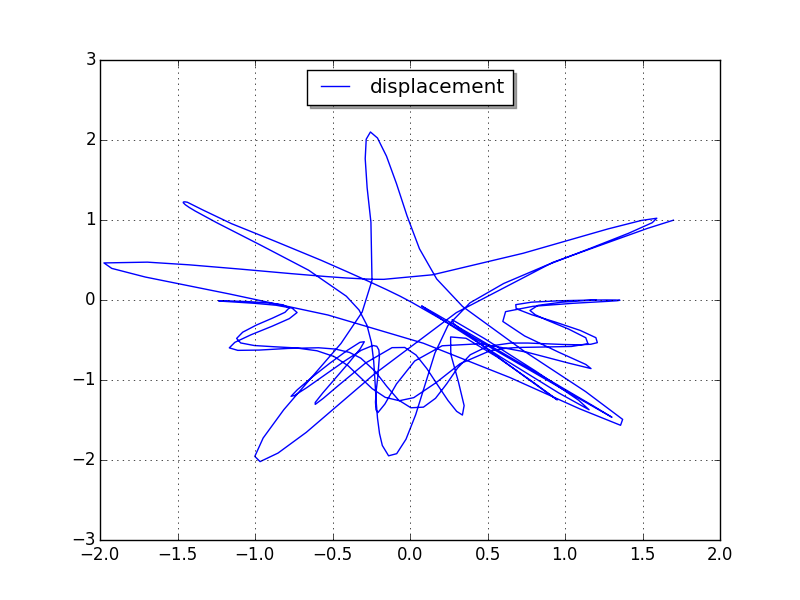
\includegraphics[scale=0.5]{task1_k50_utdrag12_rtol01.png}
\caption{tracings of the pendulum trajectory for $k = 50$ with $atol = 1$}
\label{3k10at01}
\end{figure}

\subsubsection*{MAXORD}
The maximum order still only affects the number of steps. The highly oscillating case originally takes more steps than the low oscillation (1100 steps), thus it makes sense that when using maximum order 1 we get about twice as many steps compared to the low oscillation case (76856 steps)

\subsubsection*{Choice of discretization}


\section*{Task 5} 
%DYMOLA MODELLICA
\begin{tabular}{| l | c | c |}
\hline
 Method \textbackslash \, Program & Assimulo & Dymola \\ \hline
 & \begin{tabular}{c | c | c | c}
  steps & calls & J-eval & nonlinear
 \end{tabular}
 & \begin{tabular}{c | c | c | c}
  steps & calls & J-eval & nonlinear
 \end{tabular} \\ \hline
 Euler & \begin{tabular}{c | c | c | c}
  1 & 1 & 1 & 1
 \end{tabular}
  & \begin{tabular}{c | c | c | c}
  1 & 1 & 1 & 1
 \end{tabular} \\ \hline
 BDF2 & \begin{tabular}{c | c | c | c}
  1 & 1 & 1 & 1
 \end{tabular}
 & \begin{tabular}{c | c | c | c}
  1 & 1 & 1 & 1
 \end{tabular} \\ \hline
 BDF3 & \begin{tabular}{c | c | c | c}
  1 & Van Slooten & 1 & 1
 \end{tabular}
 & \begin{tabular}{c | c | c | c}
  1 & 1 & 1 & 1
 \end{tabular} \\ \hline
 BDF4 & \begin{tabular}{c | c | c | c}
  1 & 1 & 1 & 1
 \end{tabular}
 & \begin{tabular}{c | c | c | c}
  1 & 1 & 1 & 1
 \end{tabular} \\ \hline
 CVODE & \begin{tabular}{c | c | c | c}
  1 & 1 & 1 & 1
 \end{tabular}
 & \begin{tabular}{c | c | c | c}
  1 & 1 & 1 & 1
 \end{tabular} \\ \hline
 
\end{tabular}

%x = 1.2, k = 10, Atol = 1e-6, Rtol = 1e-6

\section*{Task 6}
%WE DID THIS
%H*R LÄG IN E NTABEL OM MED CAPTIONS TYP ALLA PARMATTERRA RO SÅNT

\end{document}